\documentclass[aspectratio=169]{beamer}


\usepackage[brazil]{babel}
\usepackage[utf8]{inputenc}
\usepackage{algorithm, algpseudocode}
\usepackage{graphicx}
\usepackage{subfig}
\usepackage{multicol}
\usepackage{verbatim}
\usepackage[absolute]{textpos}
\usepackage{todonotes}\presetkeys{todonotes}{inline}{}
\usepackage{minted}
\usepackage{xcolor}
\makeatletter
\renewcommand{\ALG@beginalgorithmic}{\small}
\makeatother

\usetheme[progressbar=foot]{metropolis}

\title{Sistemas Embutidos (Avançados)}
\subtitle{Síntese em \textit{Hardware} Reconfigurável}
\date{Última Atualização: \today}
\author{Rodolfo Labiapari Mansur Guimarães}

\institute{
	\textit{rodolfolabiapari@gmail.com} \\
	Lattes: \url{http://goo.gl/MZv4Dc} \\
	Departamento de Computação -- Universidade Federal de Ouro Preto \\
		Ouro Preto - MG -- Brasil }



\begin{document}
\maketitle

\usebackgroundtemplate{
\includegraphics[trim=0 245cm 0 0, width=0.05\textwidth]{img/ufop.jpg}}

\section{Livro Texto: \\ \it{Embedded Systems Design with Platform FPGAs} \cite{Sass2010}}
	\begin{frame}
		\begin{figure}[h]
			\centering
			\caption{Livro Texto: \textit{Embedded Systems Design with Plataform FPGAs: Principles and Practices}.}
			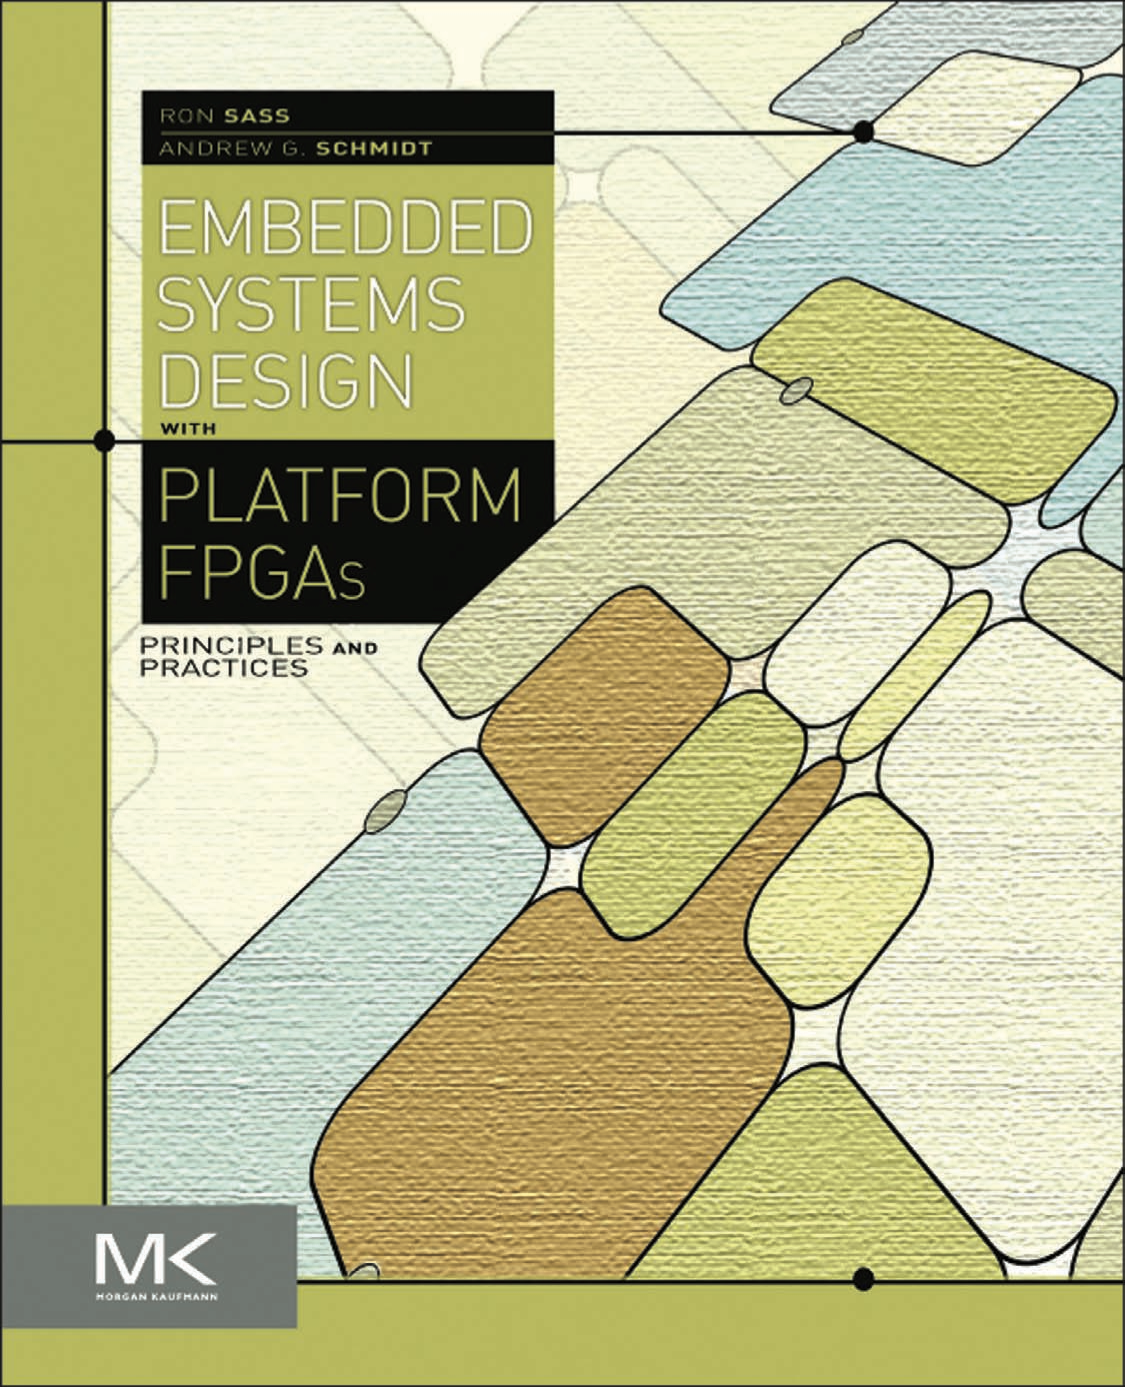
\includegraphics[height=0.89\textheight]{img/book.png}
			\label{fig:ed-tabela_verdade}
		\end{figure}
	\end{frame}
	
	\begin{frame}{O Que Será Abordado?}
		\begin{enumerate}
			\item \textit{Programmable Logic Devices} (PLD);
			\item Propriedades do FPGA;
			\item Escrita em VHDL para FPGAs.
		\end{enumerate}
	\end{frame}

\section{Introdução}
	\begin{frame}{Introdução}
		
		\begin{figure}[h]
			\centering
			\caption{``FPGA é um \textbf{quadro negro} que pode ser \textbf{desenhado} qualquer circuito digital''.}
			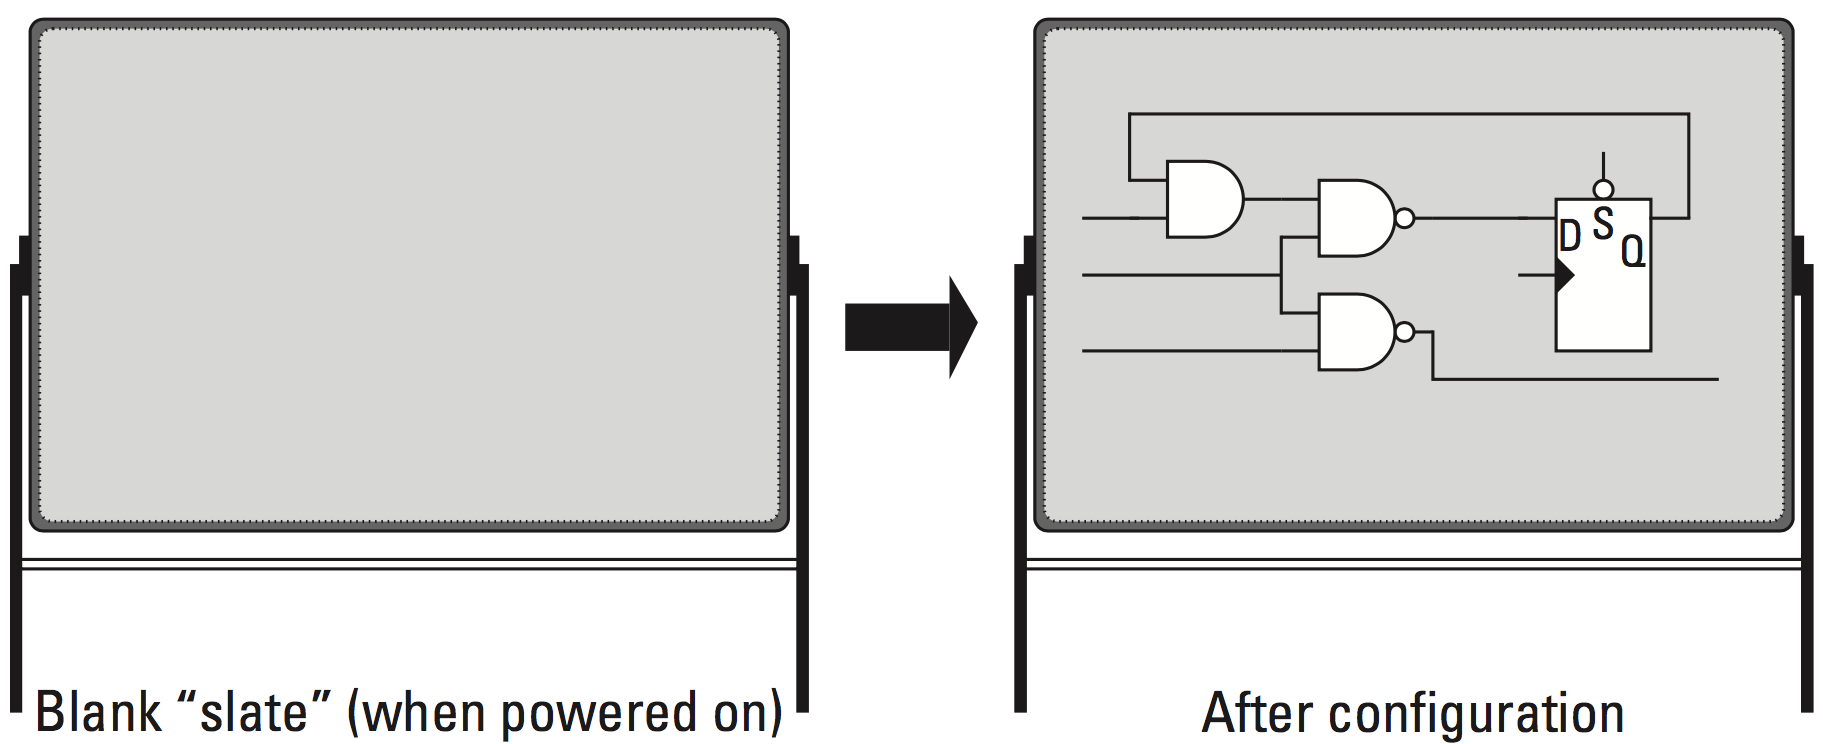
\includegraphics[height=0.7\textheight]{img/print/quadro.png}
			\label{fig:quadro}
		\end{figure}
	\end{frame}
	
	
\section{\it{Embedded Systems}}

\begin{comment}
	\begin{frame}[allowframebreaks]{Embedded Systems -}
		\begin{itemize}
			\item Diferenciação de Sistema Embarcado com Propósito Geral:
			\begin{itemize}
				\item SE: 
				\begin{itemize}
					\item Sistema de propósito específico/dedicado.
					\item O usuário não interage diretamente, ou possui interface limitada (como ser controlado remotamente).
					\item Exemplos: MP3 Player.
				\end{itemize}
				\item PG: 
				\begin{itemize}
					\item Suas entradas e saídas são poucas e padronizadas, (mouse, teclado, internet).
					\item Possuem um sistema operacional, linguagens de programação, arquiteturas variadas...
					\item O usuário interage diretamente e sabe que comprou um computador.
				\end{itemize}
			\end{itemize}
			
			\item Com isso é possível perceber que o PG e o SE não são preto e branco e sim um espectro/gradiente.
			
		\end{itemize}
	\end{frame}
\end{comment}
	
	\subsection{Modelos de Execução}
	\begin{frame}{Embedded Systems - Modelos de Execução}
		\begin{itemize}
			\setlength\itemsep{1em}
			\item Um dos maiores desafios do \textit{design} de um sistema embarcado é o fato de ter \textit{hardware} e \textit{software} no \textit{design} do projeto como um todo.
			
			\item FPGA é um \textit{hardware} que é `escrito como \textit{software}'.
			
			\item Por exemplo: um \textit{software} é executado de forma sequencial e com o resultado as operações são realizadas em ordem. Entretanto, circuitos digitais são naturalmente paralelo e engenheiros devem explicitar a sincronização disso no \textit{design}.
			
			\item Para concretizar, suponha \texttt{ACC = R0+R1+R2} sendo todos os quatro, registradores.
		\end{itemize}
	\end{frame}

	\begin{frame}{Embedded Systems - Modelos de Execução}
		\begin{figure}[h]
			\centering
			\caption{Execução \textbf{sequencial} de \texttt{ACC = R0+R1+R2}.}
			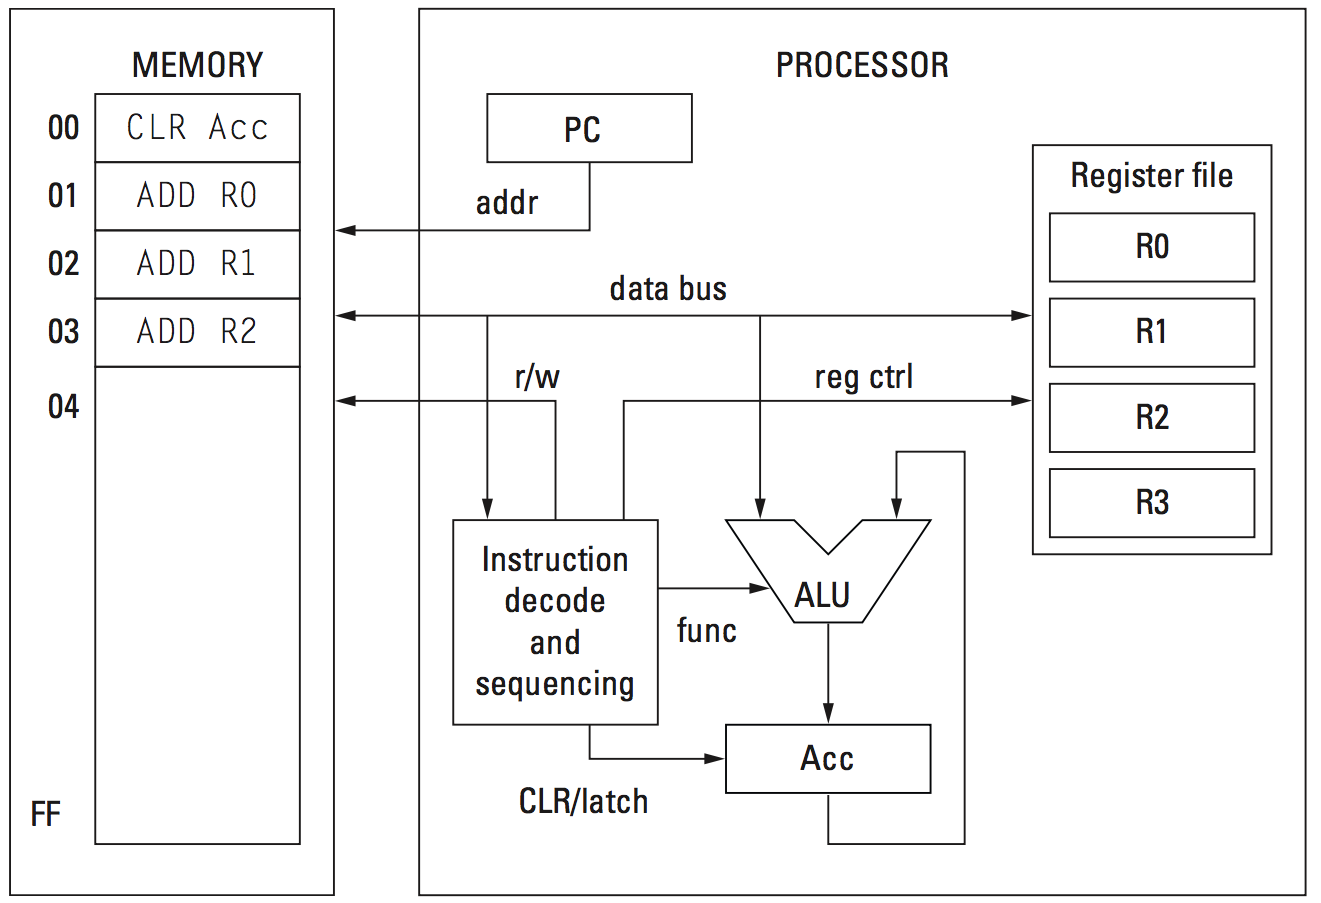
\includegraphics[height=0.8\textheight]{img/print/circuito-fixo.png}
			\label{fig:circuito-fixo}
		\end{figure}
	\end{frame}
	
	\begin{frame}{Embedded Systems - Modelos de Execução}
		\begin{figure}[h]
			\centering
			\caption{Execução da operação \texttt{ACC = R0+R1+R2} em \textbf{fluxo de dados}.}
			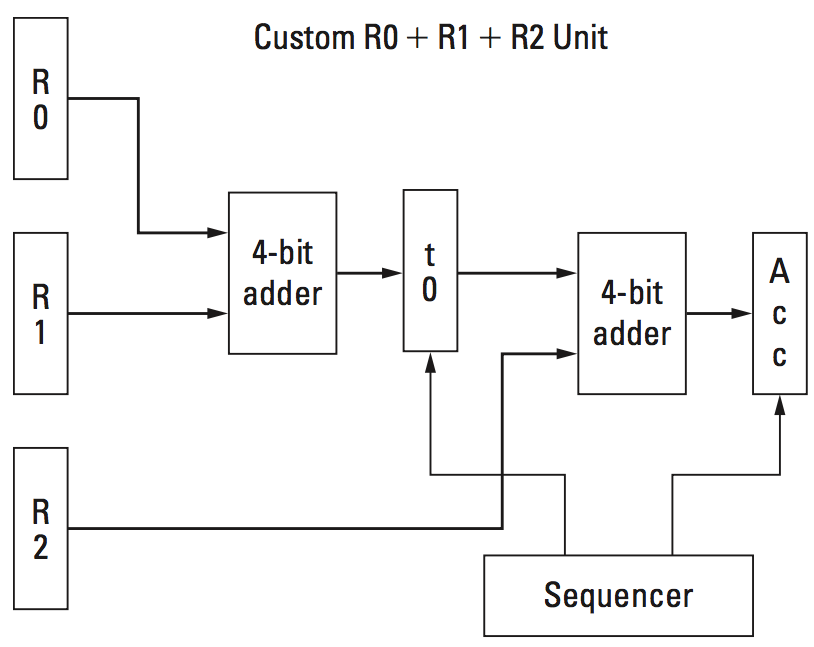
\includegraphics[height=0.8\textheight]{img/print/fluxo-dados.png}
			\label{fig:fluxo-dados}
		\end{figure}
	\end{frame}
	
	\begin{frame}%{Embedded Systems - Modelos de Execução}
			\begin{figure}[h]
				\centering
				\caption{Comparação entre ambas as execuções sobre a operação \texttt{ACC = R0+R1+R2}.}
				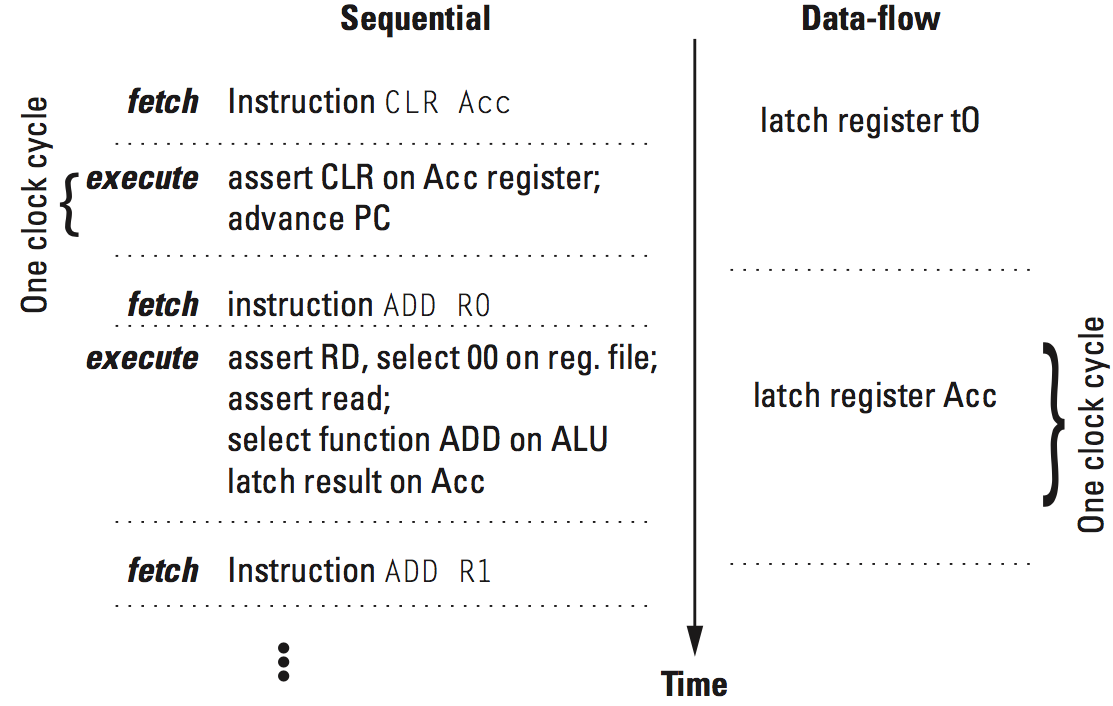
\includegraphics[height=0.7\textheight]{img/print/assembly.png}
				\label{fig:assembly}
			\end{figure}
			\pause
			\begin{block}{Questão}
				\textit{Processador executando de modo sequencial} e \textit{software executando como um processador paralelo}?
			\end{block}
	\end{frame}

\section{\it{Programmable Logic Devices} (PLD)}
	\subsection{Introdução}
	\begin{frame}{Programmable Logic Devices - Introdução}
		\begin{itemize}
			\item Transistores são \textbf{afixados} na placa no ato da fabricação.
			\begin{itemize}
				\item Uma vez afixado na placa, sua \textbf{funcionalidade} também torna \textbf{fixa}.
			\end{itemize}
		\end{itemize}
		
		\begin{block}{Questão}
			Como pode-se construir um dispositivo que seja (re)configurado mesmo \textbf{após} sua fabricação?
		\end{block}
		\pause
		\vfill
		\begin{block}{Resposta}
			Necessita-se de uma estrutura que suporte: 1) implementação de circuitos combinacionais arbitrários, 2) uma memória de armazenamento e 3) mecanismo de conexão entre eles.
		\end{block}
	\end{frame}
	
	\subsection{Programmable Logic Arrays}
	\begin{frame}{Programmable Logic Devices - Programmable Logic Arrays}
		\begin{itemize}
			\item Primeiro circuito desenvolvido.
			\item Utilizava a formulação de Soma de Produtos de uma função Booleana.
			\begin{itemize}
				\item Possui um vetor de várias entradas AND e um vetor de OR.
			\end{itemize}
		\end{itemize}
		
		
		\begin{figure}[h]
			\centering
			\caption{Abstração do \textit{Programmable Logic Arrays}.}
			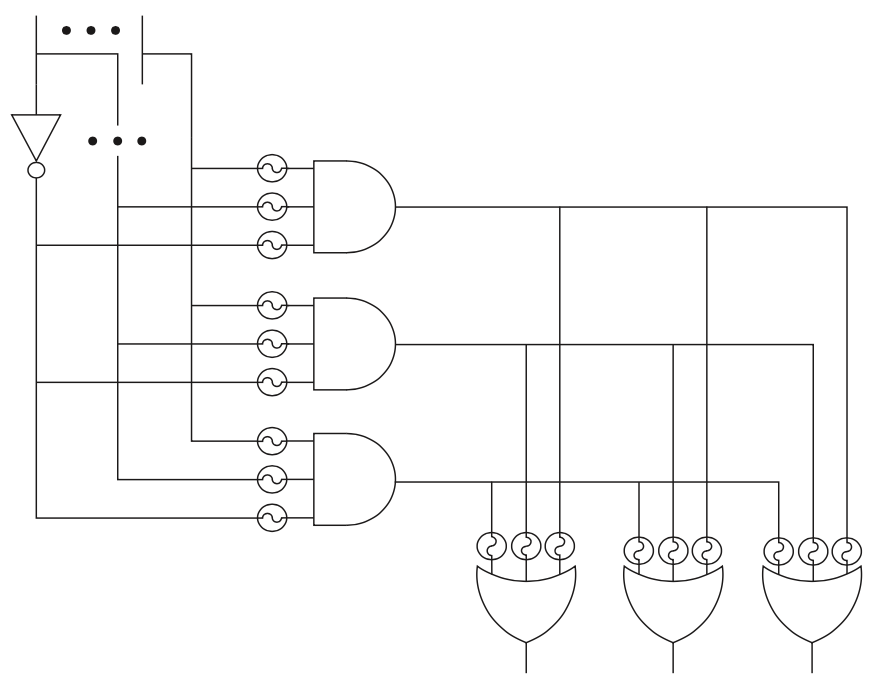
\includegraphics[height=0.57\textheight]{img/print/pla.png}
			\label{fig:pla}
		\end{figure}
	\end{frame}
	
	\subsection{Complex Programmable Logic Devices}
	\begin{frame}{Programmable Logic Devices - Complex Programmable Logic Devices}
		
		\begin{itemize}
			\item Logo em seguida, desenvolveu-se o \textit{Complex Programmable Logic Devices} (CPLDs) que replicava os blocos PLA
		\end{itemize}
		
		\begin{figure}[h]
			\centering
			\caption{Abstração do \textit{Complex Programmable Logic Devices}.}
			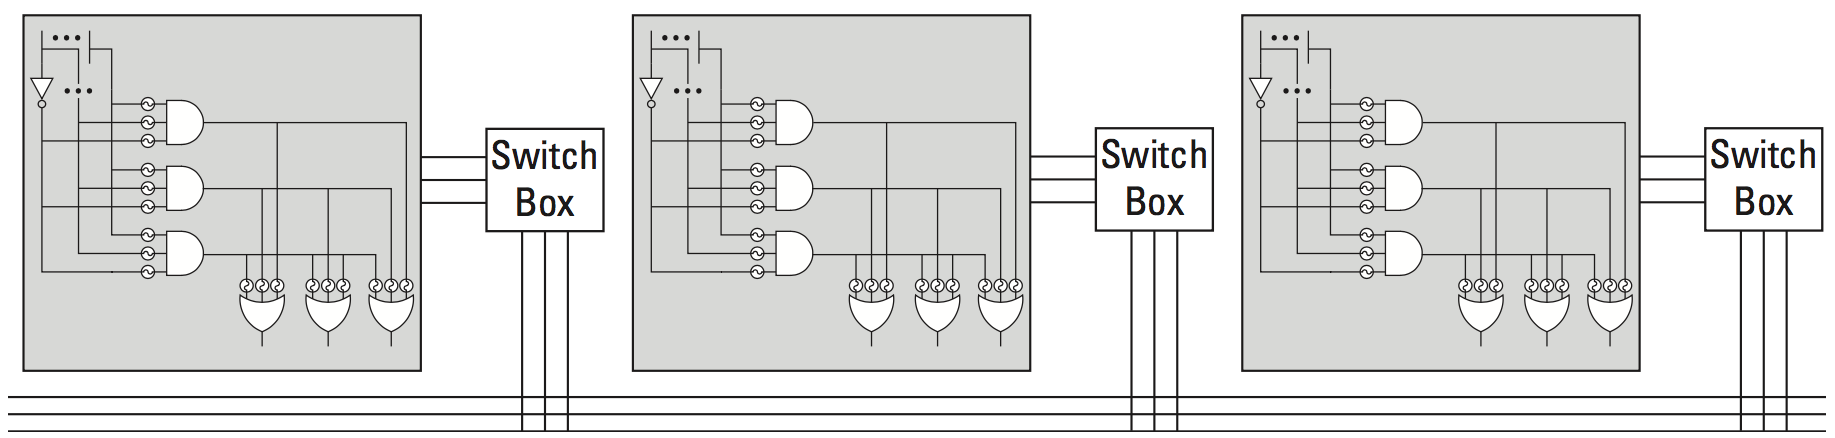
\includegraphics[height=0.42\textheight]{img/print/cpld.png}
			\label{fig:cpls}
		\end{figure}
	\end{frame}
	
\section{\it{Field-Programmable Gate Array} (FPGA)}
	\subsection{Gerador de Funções}
	\begin{frame}{Field-Programmable Gate Array (FPGA) - Gerador de Funções}
		\begin{itemize}
			\item Supondo a implementação da função Booleana $f(x, y, z) = xy + z'$.
		\end{itemize}
		
		\begin{figure}[h]
			\centering
			\caption{Gerador de Função. a) tabela verdade e b) Look-Up Table (LUT)}
			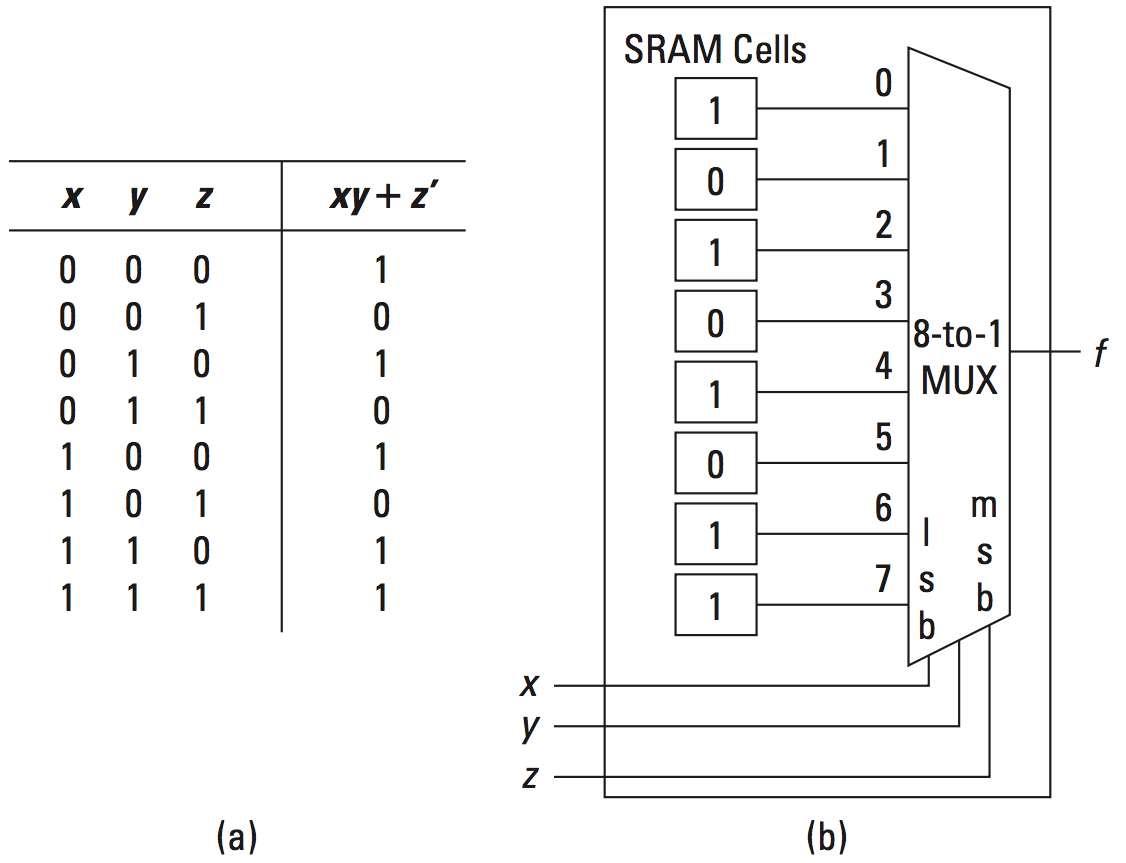
\includegraphics[height=0.68\textheight]{img/print/funcao-geradora.png}
			\label{fig:funcao-geradora}
		\end{figure}
	\end{frame}
	
	\begin{frame}{Field-Programmable Gate Array (FPGA) - Gerador de Funções}
		\begin{itemize}
			\setlength\itemsep{0.5em}
			\item Se cada saída é gravada numa memória, então basta fazer um multiplexador $8 \times 1$.
			\item É possível perceber que o \textit{delay} de cada LUT é sempre constante (o que difere dos circuitos digitais).
			\begin{itemize}
				\item Independente da complexidade dos circuitos, o atraso de propagação permanece sempre o mesmo.
				%\item Quando o circuito depende de vários LUTs, o atraso é contabilizado pela quantidade de LUTs.
			\end{itemize}
			
			\item Para implementar uma função que utilize mais entradas que uma LUT:
			\begin{itemize}
				\item Utiliza-se várias LUTs. 
				\item Cada LUTs torna resultado de uma composição.
				\begin{itemize}
					\item Sub-funções possuem sub-conjuntos de entradas.
				\end{itemize}
			\end{itemize}
		
			\item Para isso, existe recursos no FPGA para realizar a conexão entre LUTs vizinhas com o mínimo de \textit{delay}.
			
			\item Lembrando sempre que: \textbf{SRAM são voláteis}. Quando o FPGA é desligado, \textbf{tudo é perdido}. E essa capacidade de \textbf{re-escrita} é que permite sua `reconfiguração'.
		\end{itemize}
	\end{frame}
	
	\subsection{Elementos de Armazenamento}
	\begin{frame}{Field-Programmable Gate Array (FPGA) - Elementos de Armazenamento}
		\begin{itemize}
			\setlength\itemsep{1.5em}
			\item Flip-flops D são incorporados no FPGA.
			\item Tipicamente, funcionam como se fosse saídas do Gerador de Função mencionado anteriormente.
			
			\item Também, são utilizados de várias maneiras diferentes de acordo com o projeto. 
		\end{itemize}
	\end{frame}
	
	\subsection{Componentes}
	\begin{frame}{Field-Programmable Gate Array (FPGA) - Componentes}
		\begin{figure}[h]
			\centering
			\caption{Células Lógicas, Blocos Lógicos e Rede de roteamento.}
			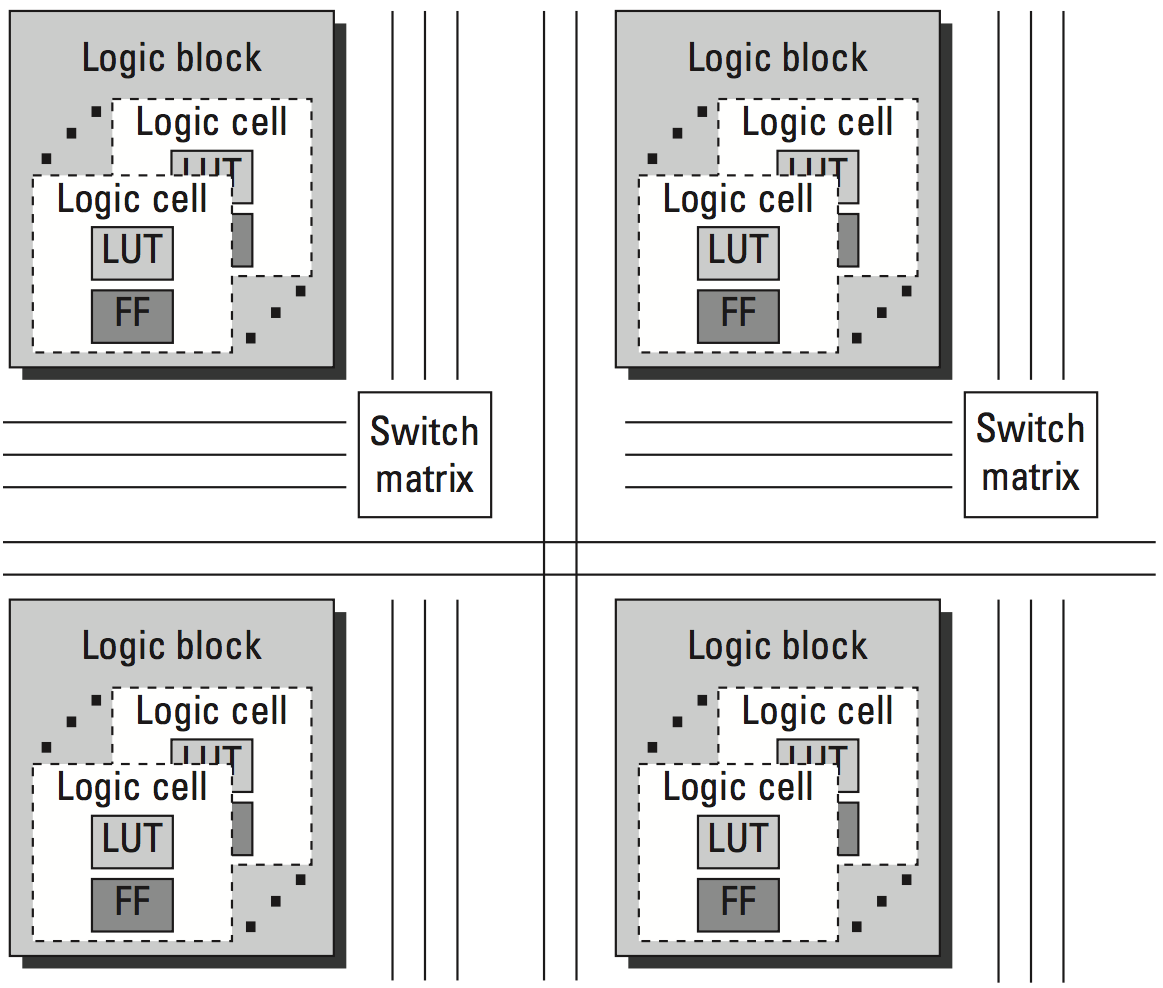
\includegraphics[height=0.8\textheight]{img/print/componentes-fpga.png}
			\label{fig:componentes-fpga}
		\end{figure}
	\end{frame}
	
	\begin{frame}{Field-Programmable Gate Array (FPGA) - Componentes}
		\begin{tabular}{cc}
			\begin{minipage}{0.35\textwidth}
				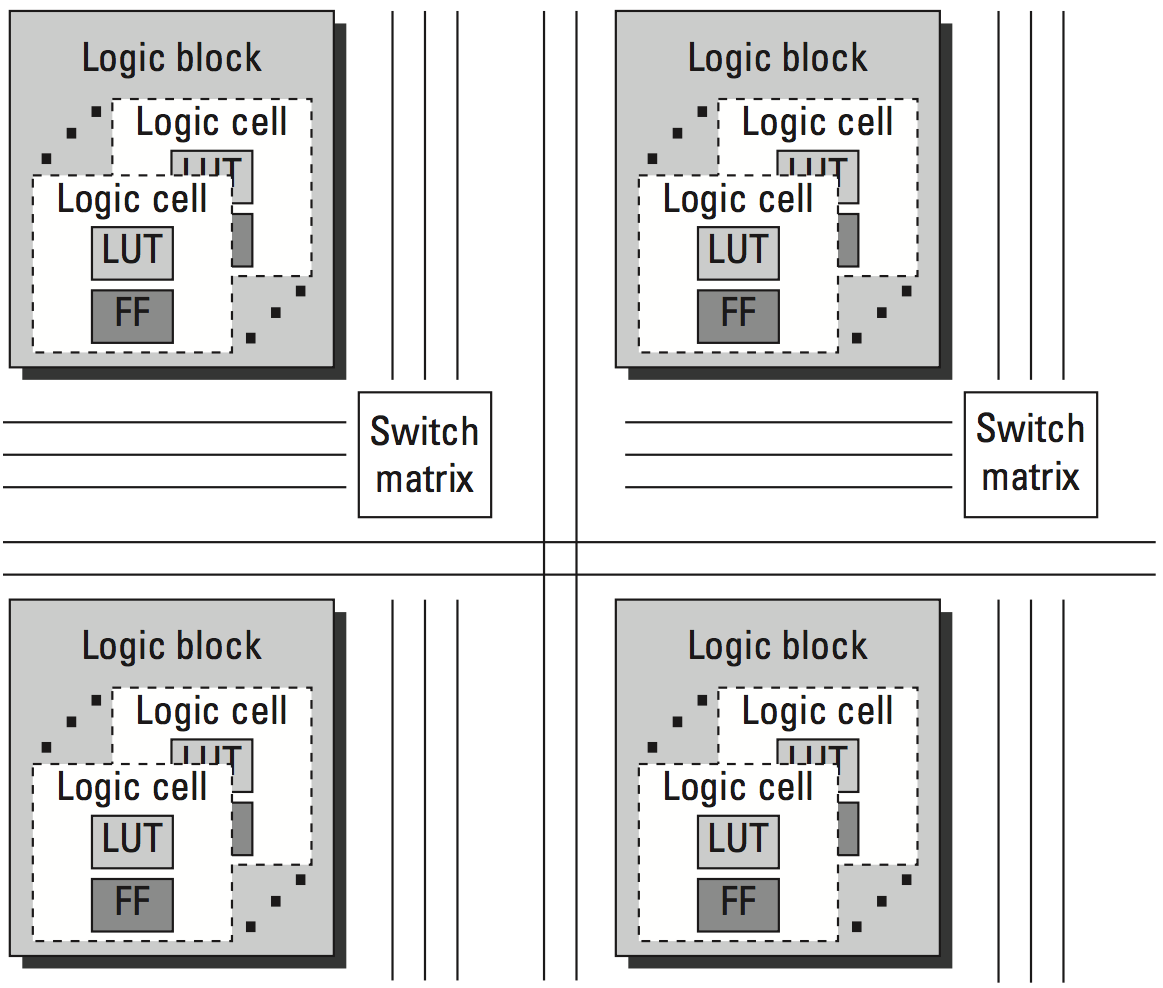
\includegraphics[height=0.62\textheight]{img/print/componentes-fpga.png}
			\end{minipage}
			&
			\begin{minipage}{0.65\textwidth}
				\begin{itemize}
					\setlength\itemsep{1.5em}
					\item Células e \textbf{Blocos Lógicos} constituem do nível mais baixo de \textit{hardware} do FPGA.
					
					\item Blocos combinacionais/sequenciais constituem células lógicas.
					
					\item Blocos Lógicos podem ser utilizados para circuitos de propósito específicos como uma pequena ALU.
					\begin{itemize}
						\item Permite que grupos lógicos de célula sejam geograficamente próximos permitindo caminhos de comunicação curtos e rápidos, e principalmente curto na implementação do \textit{design}.
					\end{itemize}
					
				\end{itemize}
			\end{minipage}
		\end{tabular}
	\end{frame}
	
	
	\begin{frame}{Field-Programmable Gate Array (FPGA) - Componentes}
		
		\begin{tabular}{cc}
			\begin{minipage}{0.35\textwidth}
				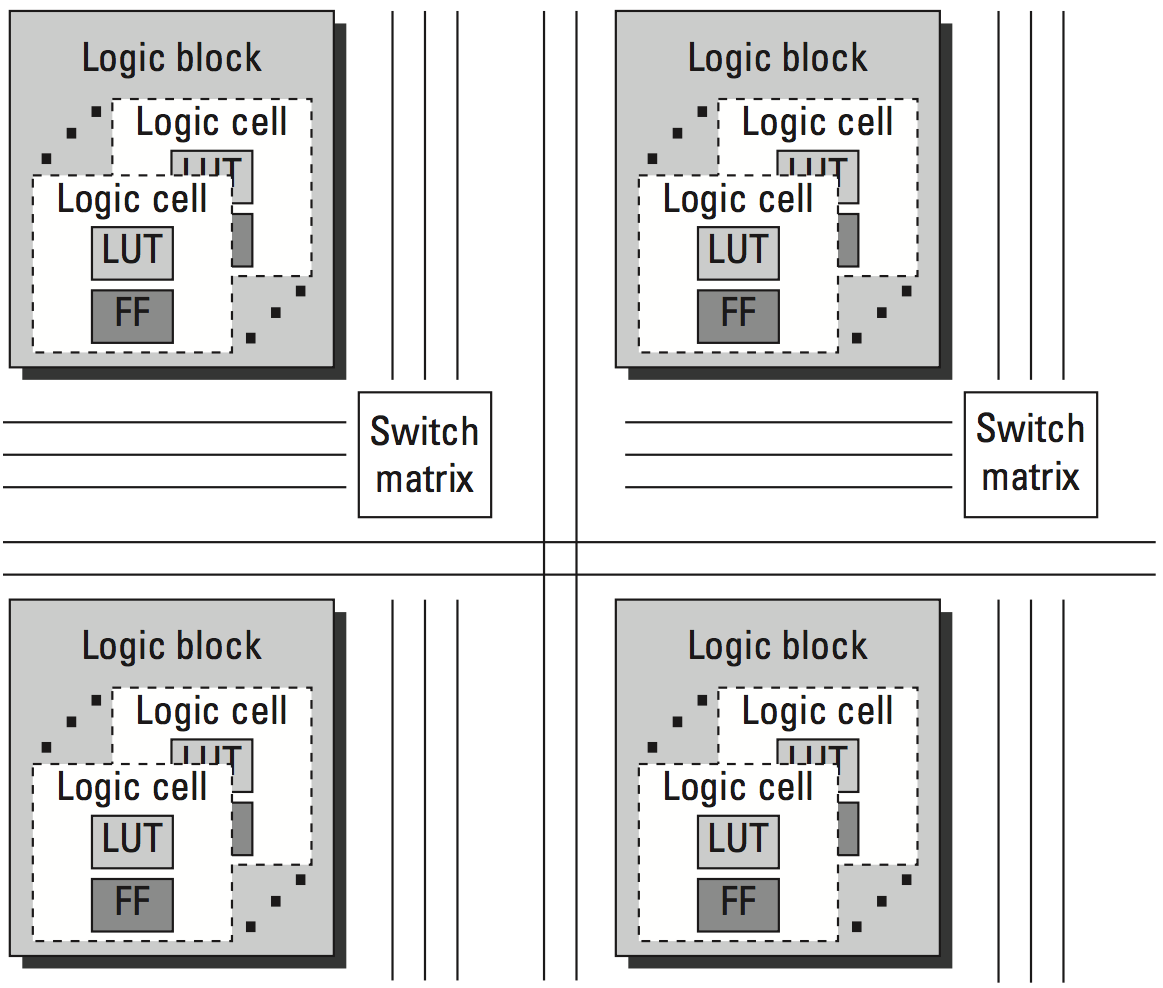
\includegraphics[height=0.62\textheight]{img/print/componentes-fpga.png}
			\end{minipage}
			&
			\begin{minipage}{0.65\textwidth}
				\begin{itemize}
					\setlength\itemsep{1em}
					\item Blocos lógicos são conectados por meio de \textbf{Redes de Roteamento} que provê suporte até para circuitos complexos.
					\begin{itemize}
						\item Roteia entradas e saídas dos blocos até o rede de roteamento geral.
						\item Realiza a passagem de sinais de um cabo para outro de outro segmento (sendo o segmento curto ou longo).
					\end{itemize}
					
					\item Como circuitos geralmente utilizam muitos blocos, eles são postos em cadeia proporcionando uma implementação potencialmente mais rápida e fácil de ser sintetizada.
					
				\end{itemize}
			\end{minipage}
		\end{tabular}
	\end{frame}
	
	\begin{frame}%{Field-Programmable Gate Array (FPGA) - Componentes}
		\begin{tabular}{cc}
			\begin{minipage}{0.5\textwidth}
				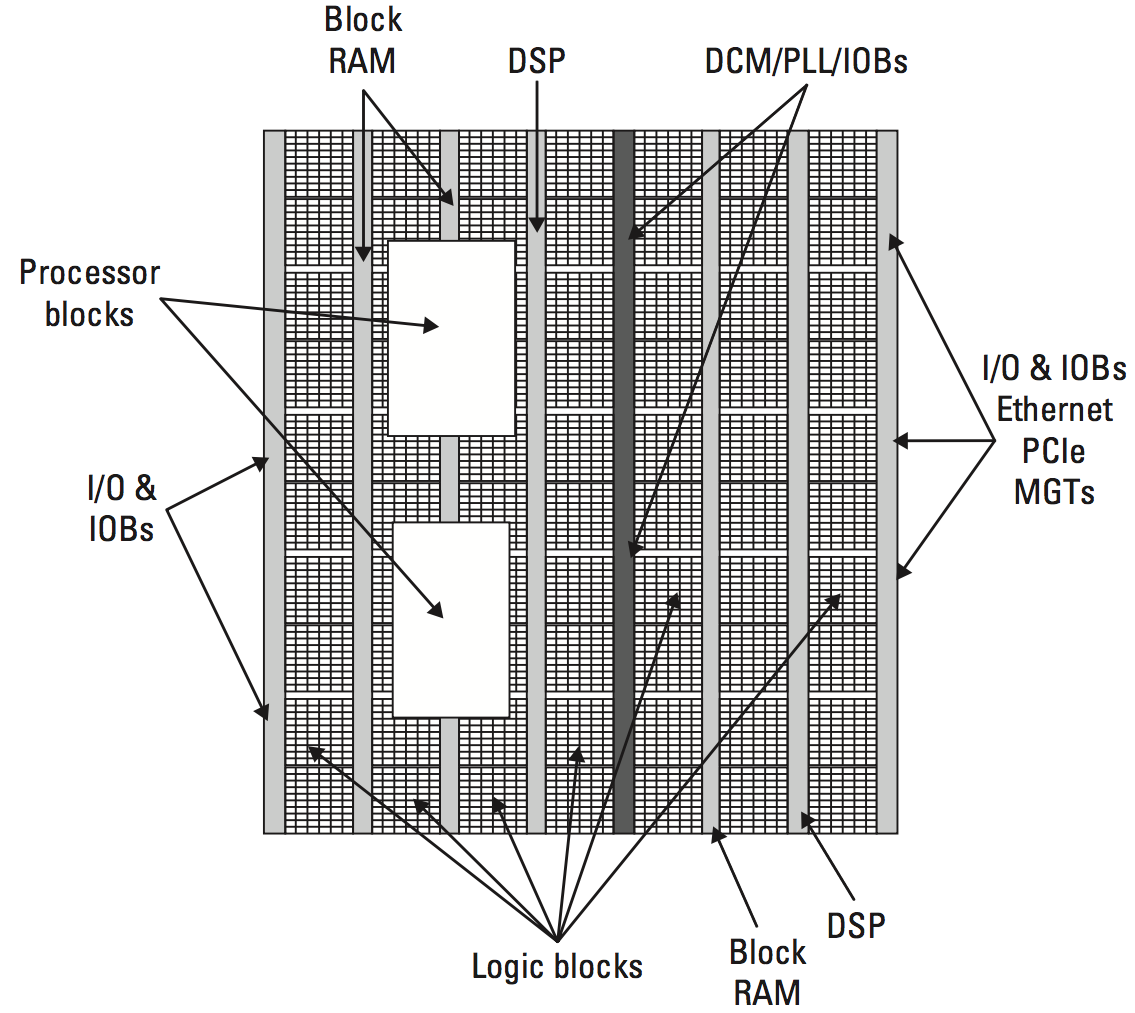
\includegraphics[height=0.92\textheight]{img/print/abstracao.png}
			\end{minipage}
			&
			\begin{minipage}{0.5\textwidth}
				\begin{itemize}
					\setlength\itemsep{1.5em}
					\item E o último é o \textbf{Bloco de I/O} (pinos).
					\begin{itemize}
						\item Ficam localizados no aborda do circuito e conectam blocos lógicos e redes de roteamento com o mundo externo.
						\item Cada pino possui sua característica especial.
					\end{itemize}
					
					\item Muitos fabricantes comparam seus FPGAs por meio de quantidade de células disponíveis.
					
					\item Com o \textbf{Bloco Lógico}, \textbf{Rede de Roteamento} e \textbf{Pinos} temos uma abstração do FPGA.
				\end{itemize}
			\end{minipage}
		\end{tabular}
	\end{frame}
	
	\begin{frame}%{Field-Programmable Gate Array (FPGA) - Componentes}
		\begin{tabular}{cc}
			\begin{minipage}{0.5\textwidth}
				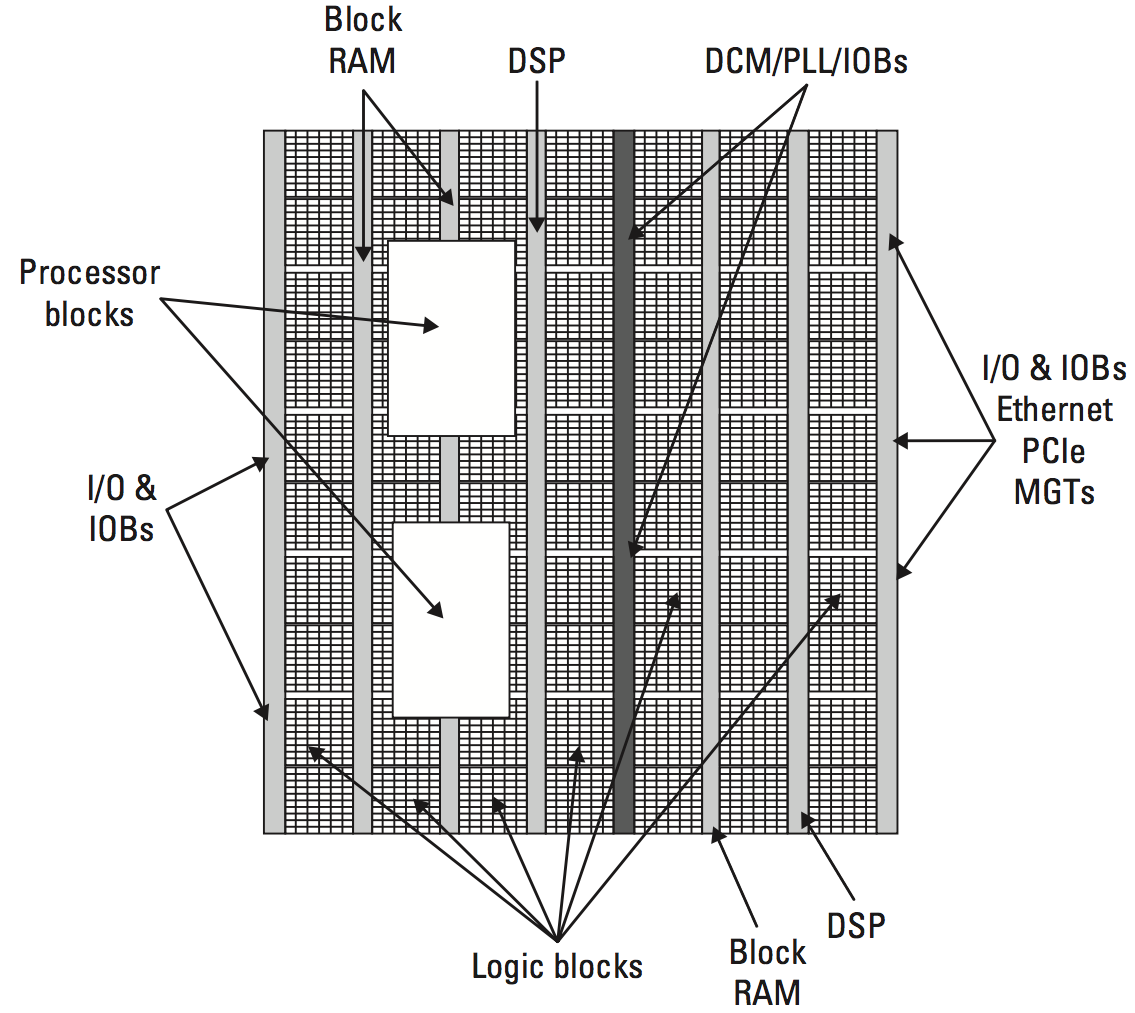
\includegraphics[height=0.9\textheight]{img/print/abstracao.png}
			\end{minipage}
			&
			\begin{minipage}{0.5\textwidth}
				\begin{block}{FPGA combina lógica programável com recursos embarcados. Porquê?}
					\begin{itemize}
						\setlength\itemsep{0em}
						\item Recursos embarcados consomem menos recursos do FPGA.
						\item Recursos embarcados consomem menos energia.
						\item Recursos embarcados podem operar com altíssima frequência.
					\end{itemize}
				\end{block}
				\begin{block}{Componentes}
					\begin{itemize}
						\setlength\itemsep{0em}
						\item \textit{Block RAM}.
						\item \textit{Digital Signal Processing Blocks}.
						\item \textit{Processors}.
						\item \textit{Digital Clock Manager}.
						\item \textit{Multi-Gigabit Transceivers}.
					\end{itemize}
				\end{block}
			\end{minipage}
		\end{tabular}
		
		\begin{itemize} \scriptsize
			\item DSP: \textit{Digital Signal Processing Blocks}.
			\item DCM, PLL: \textit{Digital Clock Manager}, \textit{Phase-locked Loop}.
		\end{itemize}
	\end{frame}

\section{\it{Hardware Description Languages} (HDL)}
	\subsection{Introdução}
	\begin{frame}{Hardware Description Languages}
		\begin{itemize}
			\setlength\itemsep{0.6em}
			\item Meio utilizado para a `configuração' de um \textit{hardware}.
			
			\item Linguagem de alto nível para descrição de circuitos digitais.
			
			\item Sua intenção inicial era para documentação e não para sintetização.
			
			\item Com o passar do tempo, foi possível ver que as linguagens poderiam ser utilizadas para simulação e consequentemente para síntese.
			\begin{itemize}
				\item Entretanto, enquanto a simulação provê um grande conjunto de recursos pra auxiliar o projetista, o mesmo não acontece na síntese.
				\item Enquanto muitas linguagens permitem a simulação, poucas fornecem recurso para síntese. Duas delas são Verilog e VHDL.
			\end{itemize}
			
			\item Existem linguagens para aumentar a produtividade como SystemC, HandelC e Impulse.
			\begin{itemize}
				\item Algumas são extensões de bibliotecas como C/C++, enquanto outras como C-like provê um ambiente mais amigável.
			\end{itemize}
		\end{itemize}
	\end{frame}
	
	\subsection{VHDL}
	\begin{frame}{Hardware Description Languages - VHSIC Hardware Description Language}
		\begin{itemize}
			\setlength\itemsep{1.8em}
			\item \textbf{VHDL:} \textbf{V}\textit{HSIC} \textbf{H}\textit{ardware} \textbf{D}\textit{escription} \textbf{L}\textit{anguage}.
			\begin{itemize}
				\item \textbf{VHSIC:} \textbf{V}\textit{ery} \textbf{h}\textit{igh-}\textbf{s}\textit{peed} \textbf{i}\textit{ntegrated} \textbf{c}\textit{ircuit}.
			\end{itemize}
			
			\item No VHDL, existe duas formas/estilos de escrever. Cada modelo tem seus impactos na síntese, simulação e em alguns caso até na produtividade. As formas são:
			\begin{itemize}
				\setlength\itemsep{0.7em}
				\item \textbf{Estrutural/Circuitos de Fluxo de Dados:} Descritos usando termos lógicos e sinais tal como AND, OR, Multiplicadores.
				\item \textbf{Circuitos Comportamentais:} Descreve em uma linguagem imperativa procedural como cada saída é relacionada com cada entrada num processo. Ideal para sistemas complexos, entretanto é possível descrever comportamentos impossíveis.
			\end{itemize}
			
			\item Exemplo de 1-bit somador completo:
		\end{itemize}
	\end{frame}
	
	\begin{frame}{Hardware Description Languages - VHDL}
		\begin{figure}[h]
			\centering
			\caption{Um 1-bit \textit{full adder} em \textbf{Tabela Verdade}.}
			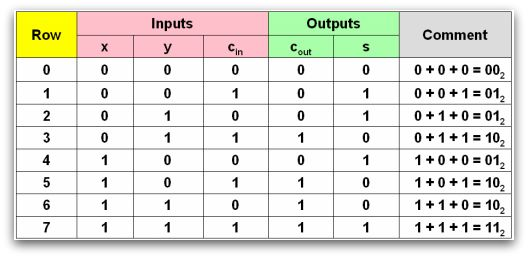
\includegraphics[height=0.9\textheight]{img/print/adder-table.jpg}
			\label{fig:tv}
		\end{figure}
	\end{frame}
	
	\begin{frame}{Hardware Description Languages - VHDL}
		\begin{figure}[h]
			\centering
			\caption{Um 1-bit \textit{full adder} em \textbf{Circuito}.}
			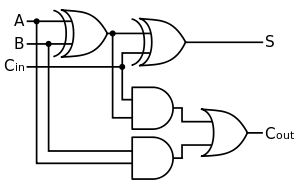
\includegraphics[height=0.8\textheight]{img/print/adder.png}
			\label{fig:ci}
		\end{figure}
	\end{frame}
	
	\begin{frame}%{Hardware Description Languages - VHDL}
		\begin{figure}[h]
			\centering
			\caption{Um 1-bit \textit{full adder} em \textbf{VHDL}.}
			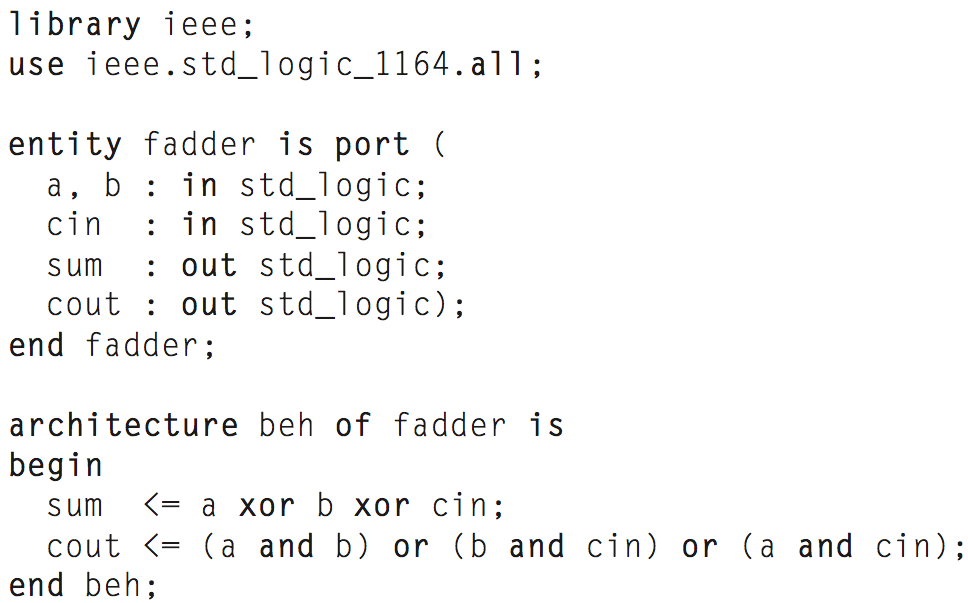
\includegraphics[height=0.92\textheight]{img/print/vhdl.png}
			\label{fig:vhdl}
		\end{figure}
	\end{frame}
	
	\begin{frame}%{Hardware Description Languages - VHDL}
		\begin{multicols}{2}
			\begin{figure}[h]
				\centering
				\caption{Um 1-bit full adder em \textbf{VHDL}.}
				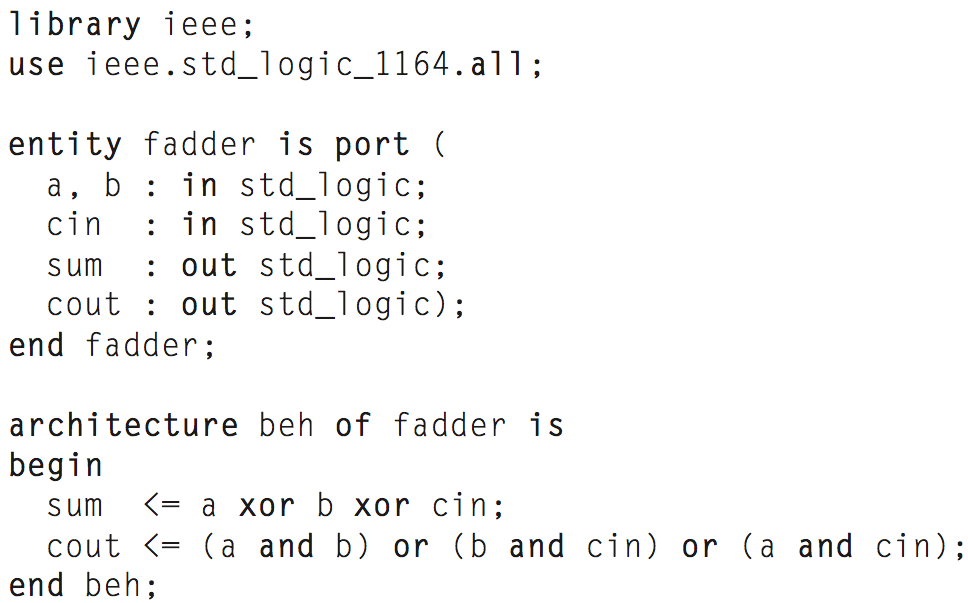
\includegraphics[height=0.85\textheight]{img/print/vhdl.png}
				\label{fig:vhdl2}
			\end{figure}
			\columnbreak
			\begin{figure}[h]
				\centering
				\caption{Um 1-bit full adder em \textbf{Circuito}.}
				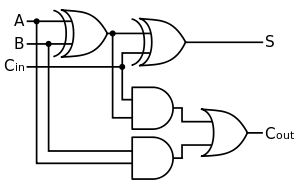
\includegraphics[height=0.6\textheight]{img/print/adder.png}
				\label{fig:ci2}
			\end{figure}
		\end{multicols}
	\end{frame}
	
	\subsection{Finite-State Machine}
	\begin{frame}{Hardware Description Languages - VHDL - FSM}
		\begin{itemize}
			\item Útil para vários propósitos.
			\item Diferentes formas de escrita resultam em diferentes sínteses.
			\item Recomenda-se seguir o guia de síntese, isto é, \textit{Xilinx Synthesis Technology (XST) User Guide}.
			\item Exemplo de somador de 8-bit:
		\end{itemize}
	\end{frame}
		
	\begin{frame}{Hardware Description Languages - VHDL - FSM}
		\textit{Livro, página 64.}
	\end{frame}
	
	\begin{frame}{Hardware Description Languages - VHDL - FSM}
		\begin{figure}[h]
			\centering
			\caption{Exemplo abstrato de uma máquina de estado.}
			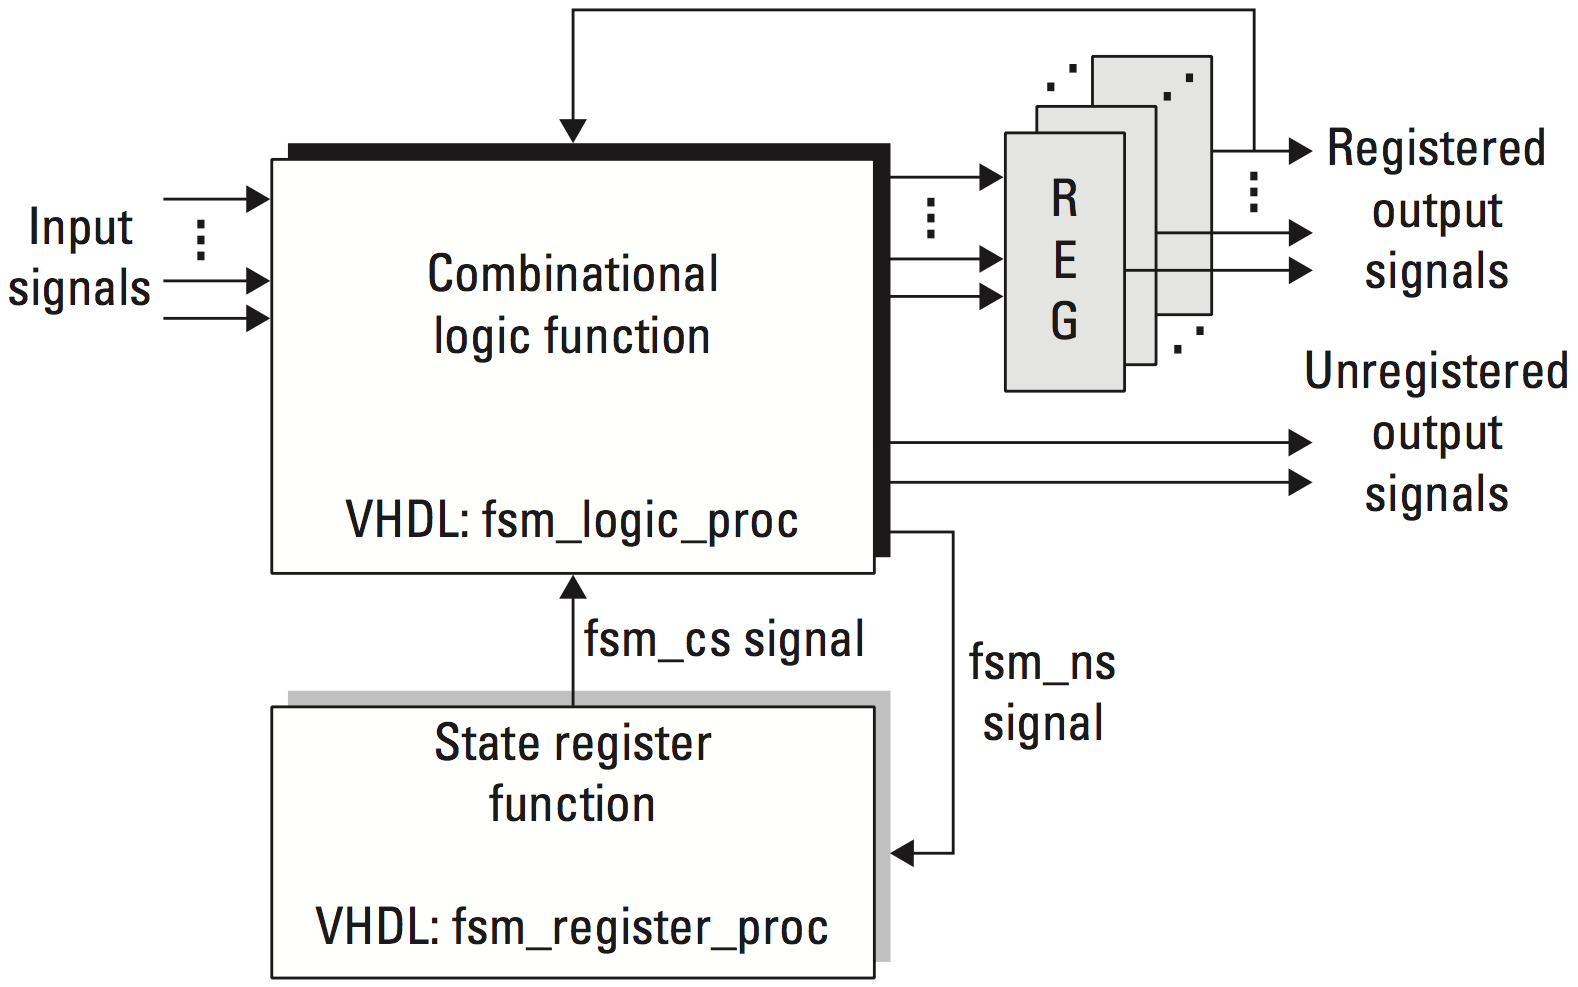
\includegraphics[height=0.77\textheight]{img/print/fsm.png}
			\label{fig:fsm}
		\end{figure}
	\end{frame}

\maketitle


\section{Bibliografia}

\bibliographystyle{abbrv}
\bibliography{sbc-template}

\maketitle

\end{document}
